\section{Empirical Results}
\label{sec:results}

\subsection{Overall Benchmark Results across Twelve Systems}
\label{sec:results:benchmark}
Table~\ref{tab:main} presents the 12-configuration benchmark across lexical (BM25), dense bi-encoder (BGE-M3), and cross-encoder reranking tiers. 
At reranking, \lineH\ achieves the highest overall retrieval effectiveness ($\text{NDCG@10} = 0.621$, 95\% CI $[0.555, 0.682]$), Top-1 accuracy ($\text{NDCG@1} = 0.800$), and reciprocal rank ($\text{MRR@10} = 0.950$). 
\lineN\ follows with $\text{NDCG@10} = 0.580$ ($[0.505, 0.649]$), while \astH\ reaches $0.487$ ($[0.419, 0.551]$), and \astN\ drops to $0.341$ ($[0.263, 0.421]$).

\begin{table}[t]
\caption{Retrieval effectiveness across 12 configurations ($N=25$ JDs).}
\label{tab:main}
\centering\scriptsize
\setlength{\tabcolsep}{2.5pt}
\begin{threeparttable}
\begin{tabular}{@{}lllccccc@{}}
\toprule
Tier & Chunk & Header & NDCG@10 [95\% CI] & NDCG@1 & MRR@10 & bpref & J@10 \\
\midrule
\multicolumn{8}{@{}l}{\textit{Two-Stage Re-ranking Tier (Cross-Encoder)}} \\
Rerank & Line & Yes & \textbf{0.621} [0.555, 0.682] & \textbf{0.800} & 0.950 & \textbf{0.353} & 0.736 \\
Rerank & Line & No & \textit{0.580} [0.505, 0.649] & \textbf{0.800} & \textbf{0.953} & \textit{0.300} & 0.716 \\
Rerank & AST & Yes & 0.487 [0.419, 0.551] & 0.740 & 0.896 & 0.241 & 0.660 \\
Rerank & AST & No & 0.341 [0.263, 0.421] & 0.340 & 0.699 & 0.170 & 0.712 \\
\midrule
\multicolumn{8}{@{}l}{\textit{Dense Bi-Encoder Tier (BGE-M3)}} \\
Dense & Line & Yes & \textbf{0.551} [0.480, 0.619] & 0.580 & 0.883 & \textbf{0.347} & 0.752 \\
Dense & Line & No & 0.521 [0.439, 0.600] & 0.600 & 0.891 & 0.297 & 0.720 \\
Dense & AST & Yes & 0.450 [0.393, 0.506] & \textbf{0.620} & \textbf{0.910} & 0.247 & 0.692 \\
Dense & AST & No & 0.358 [0.298, 0.420] & 0.420 & 0.813 & 0.179 & 0.716 \\
\midrule
\multicolumn{8}{@{}l}{\textit{Lexical Sparse Baseline Tier (BM25)}} \\
BM25 & Line & Yes & \textbf{0.433} [0.376, 0.486] & \textbf{0.440} & \textbf{0.868} & \textbf{0.255} & 0.696 \\
BM25 & Line & No & 0.405 [0.350, 0.458] & \textbf{0.440} & 0.865 & 0.246 & 0.644 \\
BM25 & AST & Yes & 0.311 [0.243, 0.376] & 0.340 & 0.761 & 0.137 & 0.676 \\
BM25 & AST & No & 0.305 [0.236, 0.371] & 0.340 & 0.724 & 0.129 & 0.560 \\
\bottomrule
\end{tabular}
\begin{tablenotes}\scriptsize
\item[] Bold: best within tier; italic: second best (Rerank tier). Linear gain $\mathrm{rel}/\log_2(i+1)$. J@10: Judged@10 coverage.
\end{tablenotes}
\end{threeparttable}
\end{table}

Dense encoding improves NDCG@10 over BM25 by $0.118$--$0.139$ with headers, and reranking adds another $0.037$--$0.070$. 
Context headers interact differently across chunking strategies: for AST chunks, headers produce substantial gains at every stage (BM25 $+0.006$, dense $+0.092$, rerank $+0.146$), whereas for line windows, gains are modest ($+0.028$, $+0.030$, $+0.041$). 
Because pooling spanned all 12 systems at top-5, $\text{Judged@5}$ is $100.0\%$ for all configurations. 
Binary preference (\texttt{bpref}) rankings perfectly mirror NDCG@10 across all tiers ($\text{Line+H}: 0.353 > \text{Line No-H}: 0.300 > \text{AST+H}: 0.241 > \text{AST No-H}: 0.170$), confirming robustness to unjudged items at deeper ranks.

\subsection{Hypothesis Testing and RQ Analyses}
\label{sec:results:hypotheses}
Table~\ref{tab:statistical_hypothesis_tests} reports the pre-specified confirmatory Wilcoxon signed-rank tests with Holm-Bonferroni correction, alongside the exploratory contrast.

\begin{figure}[t]
\centering
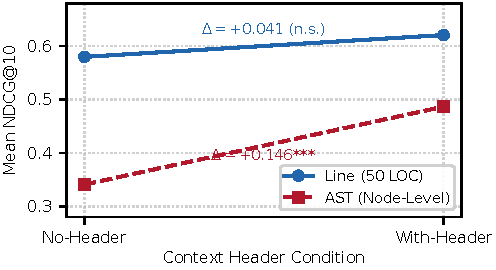
\includegraphics[width=0.72\columnwidth]{figs/fig1.pdf}
\caption{Interaction plot of context header sensitivity at reranking ($N=25$).}
\label{fig:interaction_plot}
\end{figure}

\begin{table}[t]
\caption{Hypothesis tests on NDCG@10 at reranking tier ($N=25$).}
\label{tab:statistical_hypothesis_tests}
\centering
\resizebox{\columnwidth}{!}{%
\begin{threeparttable}
\begin{tabular}{@{}llccc@{}}
\toprule
ID & Contrast ($A - B$) & $\Delta$ [95\% CI] & W/L/T & $p_{\mathrm{Holm}}$ \\
\midrule
\multicolumn{5}{@{}l}{\emph{Confirmatory family (step-down Holm, $\alpha = 0.05$)}} \\
Comp 1 & \astH\ vs. \lineN & $-0.093$ $[-0.164, -0.023]$ & 7/18/0 & $0.0438^{*}$ \\
Comp 2 & \astN\ vs. \lineN & $-0.239$ $[-0.292, -0.185]$ & 2/23/0 & $<0.001^{***}$ \\
Comp 3 & \astH\ vs. \astN & $+0.146$ $[+0.086, +0.207]$ & 23/2/0 & $<0.001^{***}$ \\
Comp 4 & \lineH\ vs. \lineN & $+0.041$ $[-0.012, +0.093]$ & 15/10/0 & $0.2411$ \\
\midrule
\multicolumn{5}{@{}l}{\emph{Exploratory (outside the Holm family)}} \\
Comp 5 & \astH\ vs. \lineH & $-0.134$ $[-0.199, -0.070]$ & 5/20/0 & $0.0003^{\dagger}$ \\
\bottomrule
\end{tabular}
\begin{tablenotes}\scriptsize
\item[] W/L/T: queries where $A$ wins, loses, or ties against $B$. Significance follows $p_{\mathrm{Holm}}$ (*~$<0.05$, **~$<0.01$, ***~$<0.001$). $^{\dagger}$~Unadjusted $p$ (exploratory).
\end{tablenotes}
\end{threeparttable}%
}
\end{table}


\textbf{RQ1 (Context Headers):} Prepending headers yields a large, significant gain for AST chunks (\textbf{Comp 3}: $\Delta = +0.146$, 95\% CI $[+0.086, +0.207]$, $p_{\mathrm{Holm}} = 0.0001$, $W = 24.0$; AST+H wins 23/25 JDs). In contrast, prepending headers to line windows yields a minor, non-significant gain (\textbf{Comp 4}: $\Delta = +0.041$, 95\% CI [$-0.012$, $+0.093$], $p_{\mathrm{Holm}} = 0.2411$, $W = 118.0$; 15 wins vs. 10 losses). As shown in Fig.~\ref{fig:interaction_plot}, headers act as vital anchors for fine-grained AST chunks while providing diminishing returns for 50-line windows.

\textbf{RQ2 (AST vs. Line):} Simple line windows without headers significantly outperform AST chunks with headers (\textbf{Comp 1}: $\Delta = -0.093$, 95\% CI [$-0.164$, $-0.023$], $p_{\mathrm{Holm}} = 0.0438$, $W = 78.0$; Line wins 18 vs. AST wins 7). Without headers, line windows strongly outperform AST chunks (\textbf{Comp 2}: $\Delta = -0.239$, 95\% CI [$-0.292$, $-0.185$], $p_{\mathrm{Holm}} < 0.001$, $W = 3.0$; Line wins 23/25). In the exploratory contrast with headers (\textbf{Comp 5}), line windows remain significantly superior ($\Delta = -0.134$, 95\% CI [$-0.199$, $-0.070$], $p_{\mathrm{raw}} = 0.0003$, $W = 36.0$; Line wins 20 vs. AST wins 5).

\subsection{Subgroups, Morphology Sensitivity, and Header Effects}
\label{sec:results:sensitivity}
\textbf{Subgroups \& Common Support:} Trends hold across languages: Java ($N=15$) yields Line+H $0.716$ vs. AST+H $0.583$ ($\Delta = -0.133$); React/TS ($N=10$) yields $0.478$ vs. $0.342$ ($\Delta = -0.136$). 
AST fallback is $0.0\%$ (0/438 chunks, 0/250 top-10 candidates). 
Evaluating on \textit{Common Support} (826/882 pairs where both strategies have candidate chunks, retaining 91.8\% of relevant evidence across all 25 queries) confirms that Line+H retains its statistically significant lead over AST+H ($0.600$ vs. $0.489$, $\Delta = +0.111$, $p_{\mathrm{Holm}} = 0.0036$, $W = 51.0$), while Line No-H dominates AST No-H ($0.535$ vs. $0.342$, $\Delta = +0.193$, $p_{\mathrm{Holm}} < 0.0001$, $W = 11.0$). 
Coverage accounts for only 17.3\% of the end-to-end gap ($+0.023$, $p = 0.0015$), demonstrating that Line superiority is driven primarily (82.7\%) by intrinsic contextual ranking.

\textbf{Window Overlap Sensitivity:} Suppressing intersecting 10-LOC overlapping windows from the same file in top-10 retrieval (26.4\% of Line top-10 slots involved in overlap [16.8\% redundant] vs. 0\% in AST) leaves deduplicated NDCG@10 intact: Line+H achieves $0.583$, Line No-H $0.574$, AST+H $0.482$, and AST No-H $0.341$. 
Line windows retain their significant lead (\textbf{Comp 5}: $\Delta = -0.101$, $p = 0.0013$; \textbf{Comp 1}: $\Delta = -0.092$, $p = 0.0236$), and the AST header boost remains large (\textbf{Comp 3}: $\Delta = +0.141$, $p < 0.001$).

\textbf{Qualitative Inspection of Header Lift:} Inspecting rank trajectories illustrates how headers ground isolated chunks. 
For \texttt{JD\_JAVA\_01} (\textit{"Spring Security \& JWT"}), the authenticated profile endpoint in \texttt{AccountController.java} (lines 39--64, \texttt{me()}, annotated \texttt{@SecurityRequirement}) rises from Rank~6 without header to Rank~1 with header (human relevance 2). 
For \texttt{JD\_REACT\_01} (\textit{"React Admin Dashboard \& RBAC"}), an administrative control panel in \texttt{Admin/index.tsx} (lines 544--613) jumps from Rank~13 to Rank~1 with header (relevance 2).
